% -*- coding: latin-1 -*-
\section{Pitch-detection}
RT\_LPC giver mulighed for at detektere pitch vha. autokorrelation. Vi har dog istedet implementeret average magnitude difference (AMDF) pitch detection p� baggrund af [Sayood] pp. 543. Formlen for AMDF er:

[formel],

hvor p er perioden. For hver frame analyserer vi med v�rdier af p mellem 2.5 og 19.5 ms, svarende til 860 Hz ned til 110 Hz, hvor menneskelig tale normalt befinder sig. Herefter v�lger vi den minimale AMDF-v�rdi som vores pitch.

\subsection{Stemte lyde}
I f�lgende eksempel analyseres 20 ms af 'y'-lyden i 'tydeligt'. X-aksen betegner p-v�rdien i samples, og Y-aksen betegner AMDF-v�rdien.

\begin{figure}
\begin{center}
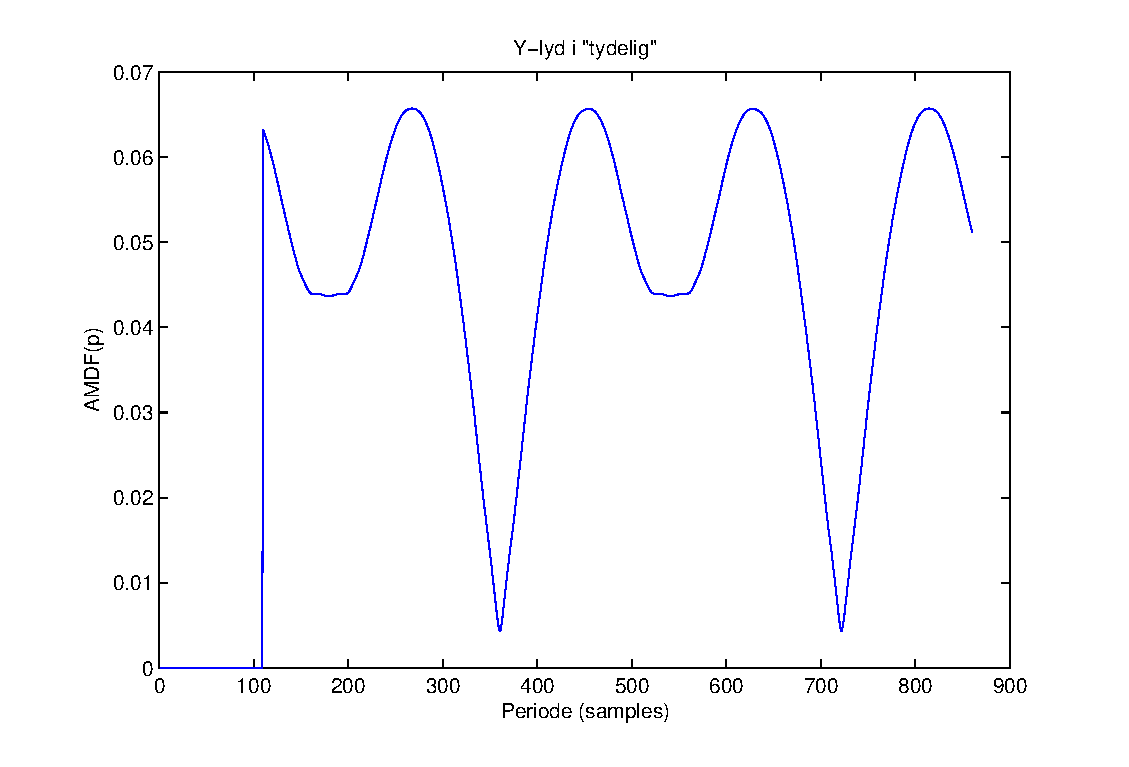
\includegraphics[width=120mm]{y-plot.eps}\\
\end{center}
\label{udstyr}
\caption{'Y'-lyd i 'tydelig'}
\end{figure}

Det ses at minimum ligger ved ca 730 samples, svarende til ca 60 Hz. Et lokalt minimum ses ved den dobbelte frekvens (den halve periode), hvilket formodentligt er en overtone.

Er den minimale v�rdi over et bestemt threshold, v�lger vi at opfatte frame'n som en ustemt lyd.

\subsection{Ustemte lyde}
I dette ekspempel analyseres 20 ms af 't'-lyden i 'tydeligt'. Det ses at alle v�rdier ligger forholdsvist samme sted p� y-aksen. Ingen v�rdi er under vores threshold og vi opfatter derfor frame'n som en ustemt lyd.

\begin{figure}
\begin{center}
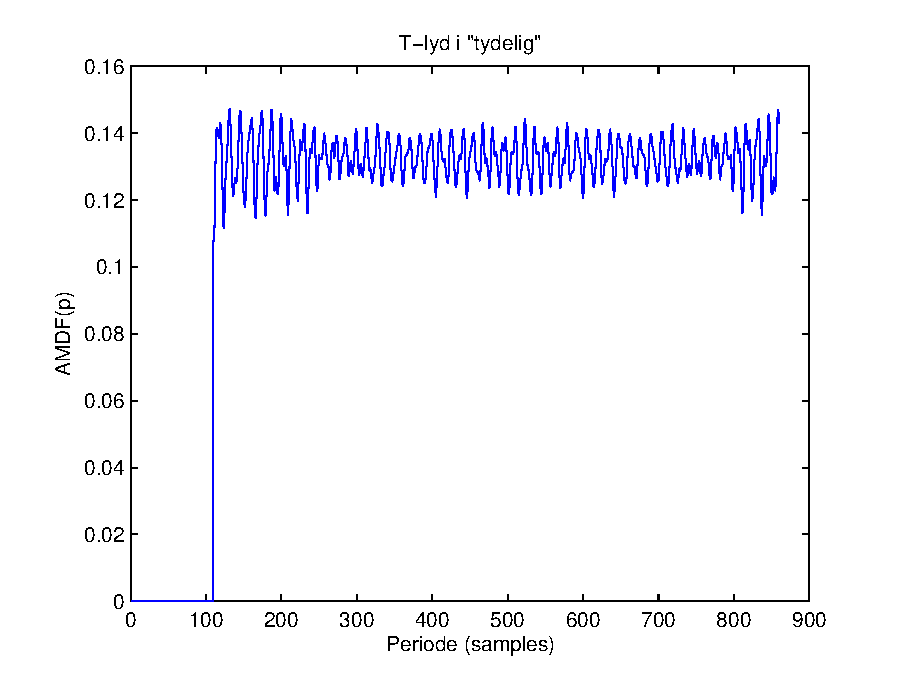
\includegraphics[width=120mm]{t-plot.eps}\\
\end{center}
\label{udstyr}
\caption{'T'-lyd i 'tydelig'}
\end{figure}

